\documentclass[a4paper, 12pt, brazilian]{article}

\usepackage{config}

\begin{document}
	\begin{titlepage}
		\begin{center}
			\begin{large}
				\textbf{Universidade Estadual de Campinas}\\\vspace{.5cm}
				\textbf{Faculdade de Engenharia Agrícola}\\\vspace{10.5cm}
			\end{large}
			\begin{large}
				\uppercase{\textbf{Compressão Uniaxial com Restrição e determinação do coeficiente de Poisson}}\\\vspace{4cm}
			\end{large}
		\end{center}
		\begin{large}
			\noindent\textbf{Nome:} \href{https://github.com/RenanSGuedes/576}{Renan da Silva Guedes}\\\\
			\noindent\textbf{RA:} 223979\\\vspace{4cm}
		\end{large}
		\begin{center}
			\begin{large}
				Campinas\\\vspace{.3cm}
				2020
			\end{large}
		\end{center}
	\end{titlepage}
	
	\newpage
	
	\section{Introdução}
	
	O ensaio a ser realizado consiste na compressão uniaxial com restrição em corpos de prova (CP) de batata inglesa, dando continuidade ao primeiro experimento. Dessa forma, a partir das repetições e procedimentos realizados, é visada a determinação do coeficiente de Poisson do material estudado.
	
	\section{Objetivos}
	
	Determinação do coeficiente de Poisson ($\nu$).
	
	\section{Materiais e Métodos}
	
	Para a realização do experimento foi feito uso das batatas, cortador cilíndrico para as mesmas, cilindro vazado para a inserção dos CPs, paquímetro digital, Máquina Universal de Ensaios e \textit{software} para aquisição de dados. 
	
	Dessa forma, após seguir os procedimentos iniciais apresentados na  \cref{fig:diagram} e realizar cinco repetições de compressão dos corpos de provas nas condições de restrição vistas no cilindro vazado, foi obtido o gráfico mostrado na \cref{fig:graph}.
	
	Feito isso, após linearizar os trechos pertinentes de cada curva, foi encontrado o parâmetro (M) a ser substituído na equação \eqref{main_eq}. Em seguida, ao fazer a interpolação dos valores de módulo de elasticidade (E) para a velocidade de
	\SI{1}{\milli\meter/\second}, baseando-se no gráfico do módulo de elasticidade em função da velocidade do primeiro ensaio (\cref{fig:interpol}), chegou-se no valor de E a ser substituído também em \eqref{main_eq}. Após obter M (coeficiente angular médio dos trechos linearizados para as cinco curvas da \cref{fig:graph}), foi possível encontrar o valor do coeficiente de Poisson para o material estudado.
	
	\section{Resultados e Discussão}
	
	Após seguir os procedimentos descritos anteriormente chegou-se que  $\textrm{E}=\SI{3.64}{\giga\pascal}$ e $\textrm{M}=\SI{5.14}{\giga\pascal}$. Consequentemente, o valor de coeficiente de Poisson atingido foi de $0.32$, contrariando os limites esperados onde $0.4<\nu<0.5$. 
	
	Tendo em vista que o coeficiente de Poisson quantifica o grau de deformação transversal e longitudinal como é visto na equação \eqref{strain}, deduz-se que o coeficiente obtido é inferior ao esperado, podendo este fato ser proveniente da deformação na direção longitudinal ($z$) ultrapassando o esperado, ou ocasionado pela nulidade das deformações transversais ($x$ e $y$) do CP pela utilização do cilindro vazado.
	
	\section{Conclusão}

	Com base no ensaio e resultados alcançados, vê-se que ocorreu redução do valor esperado para o coeficiente de Poisson. Tal fato pode estar associado à restrição incorporada ao experimento, influenciando na deformação dos CPs sob compressão.
	\section{Anexos}
	
	\subsection{Tabelas}
	
	\import{tables/}{data}
	
	\subsection{Figuras}
	
	\begin{figure}[H]
		\centering
		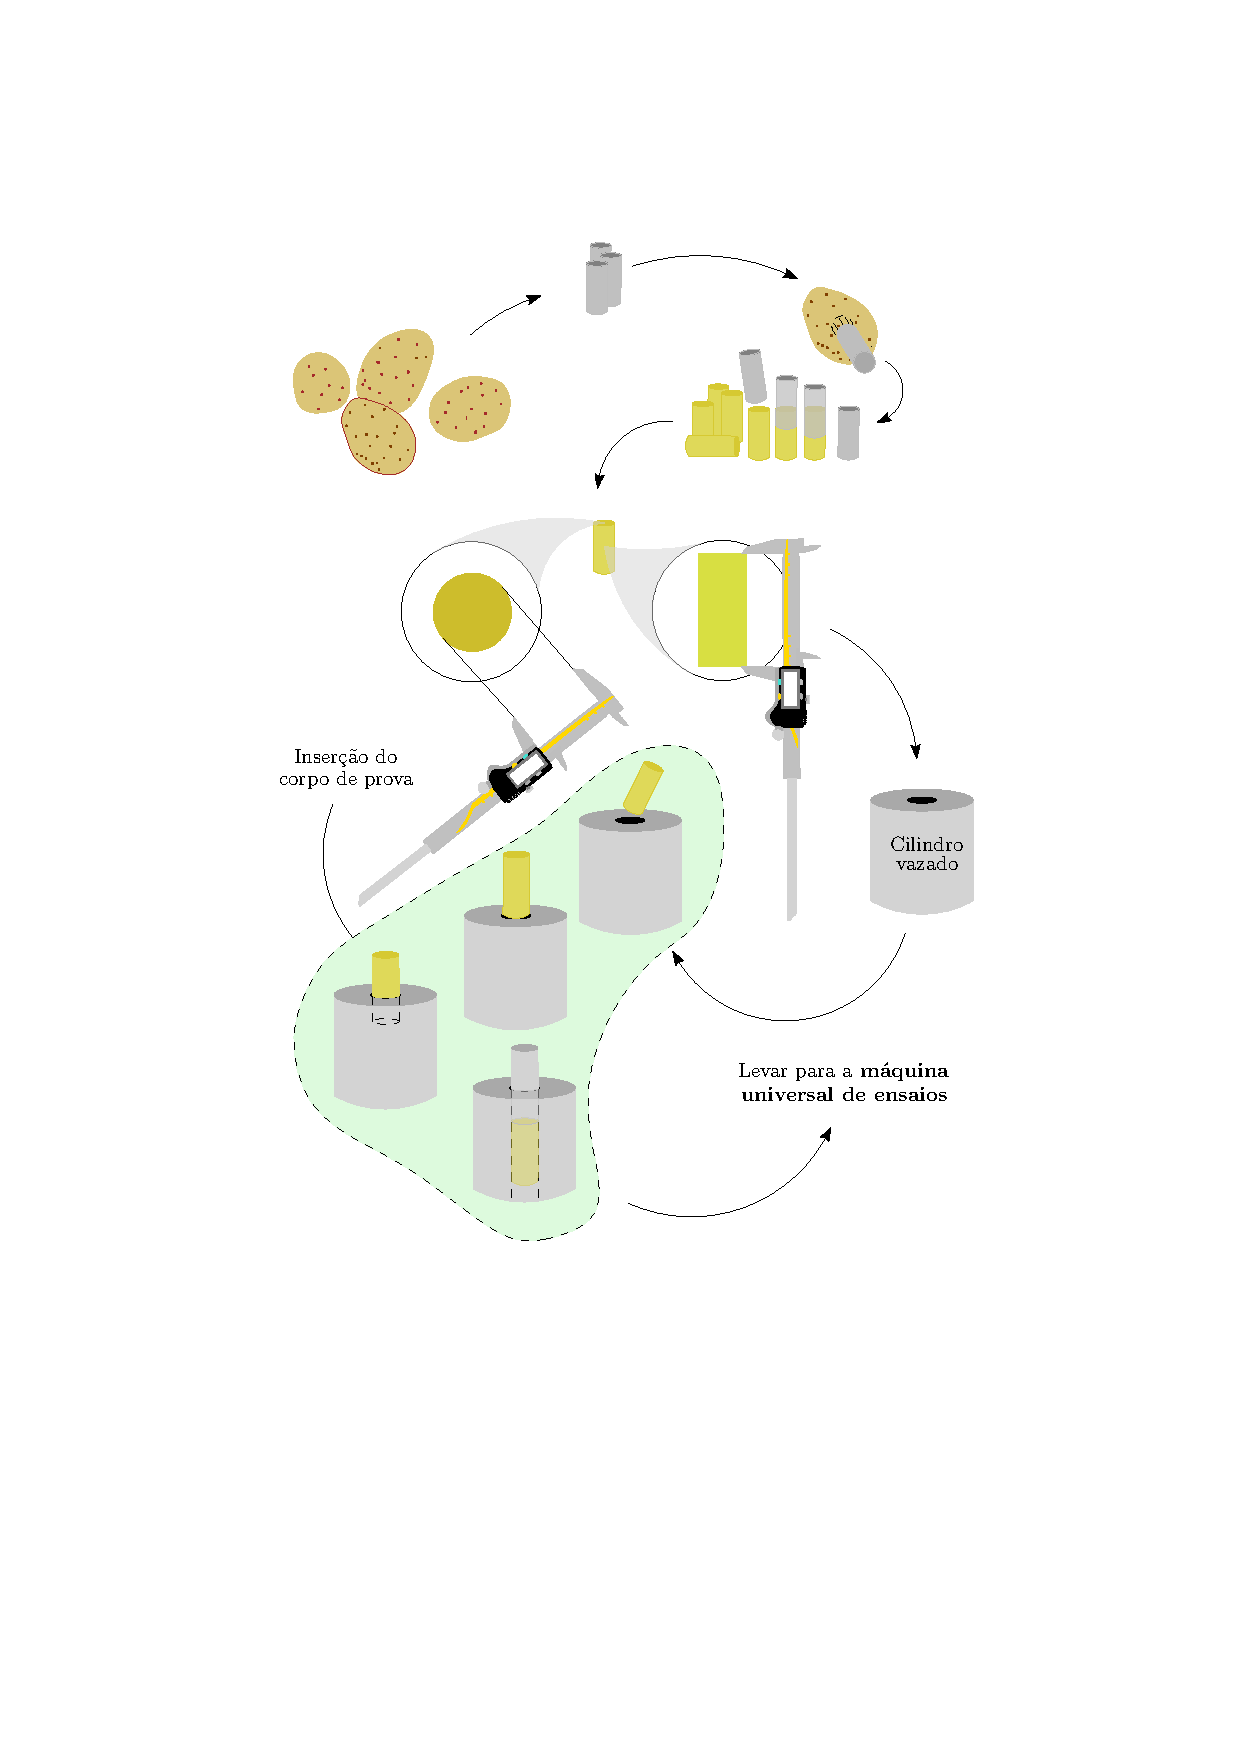
\includegraphics[scale=1.1]{images/diagram}
		\caption{Procedimentos adotados na elaboração de cada CP de batata inglesa. Após cortar a mesma no formato cilíndrico deve ser feita sua inserção no cilindro vazado seguido do cilindro atuante sobre o CP por ação da Máquina Universal de Ensaios.}
		\label{fig:diagram}
	\end{figure}

	\begin{figure}[H]
		\centering
		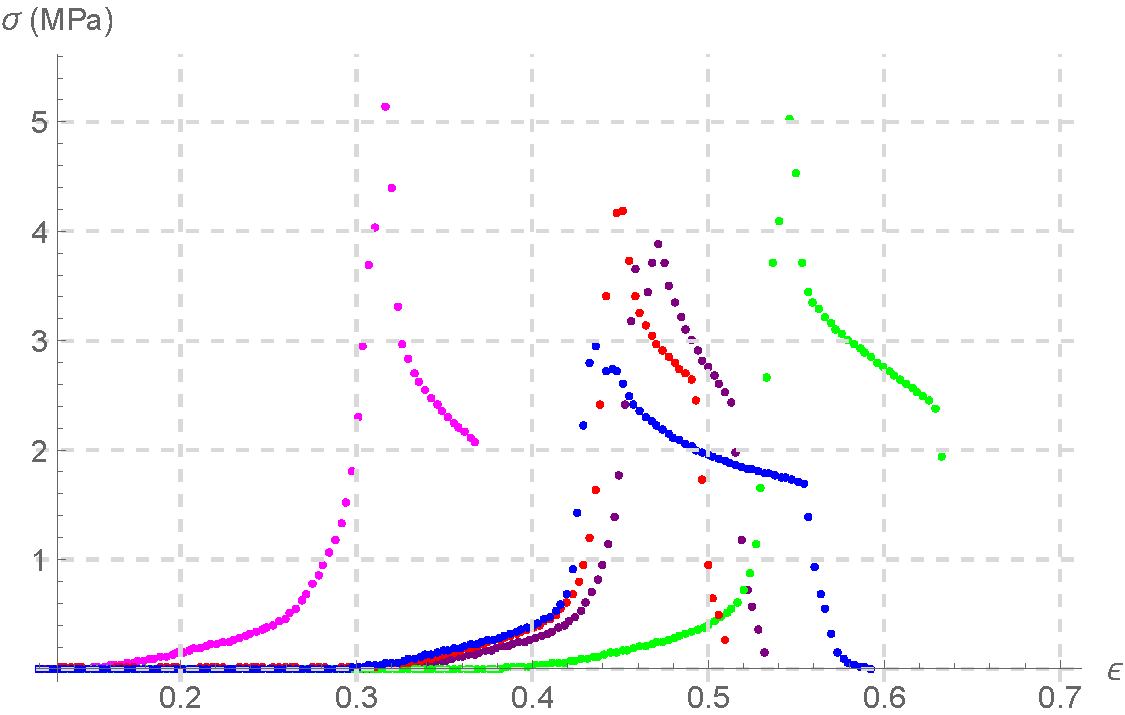
\includegraphics[scale=.6]{images/graph}
		\caption{Gráfico tensão \textit{versus} deformação para os corpos de prova sob compressão à velocidade de \SI{1}{\milli\meter/\second}.}
		\label{fig:graph}
	\end{figure}
	
	\begin{figure}
		\centering
		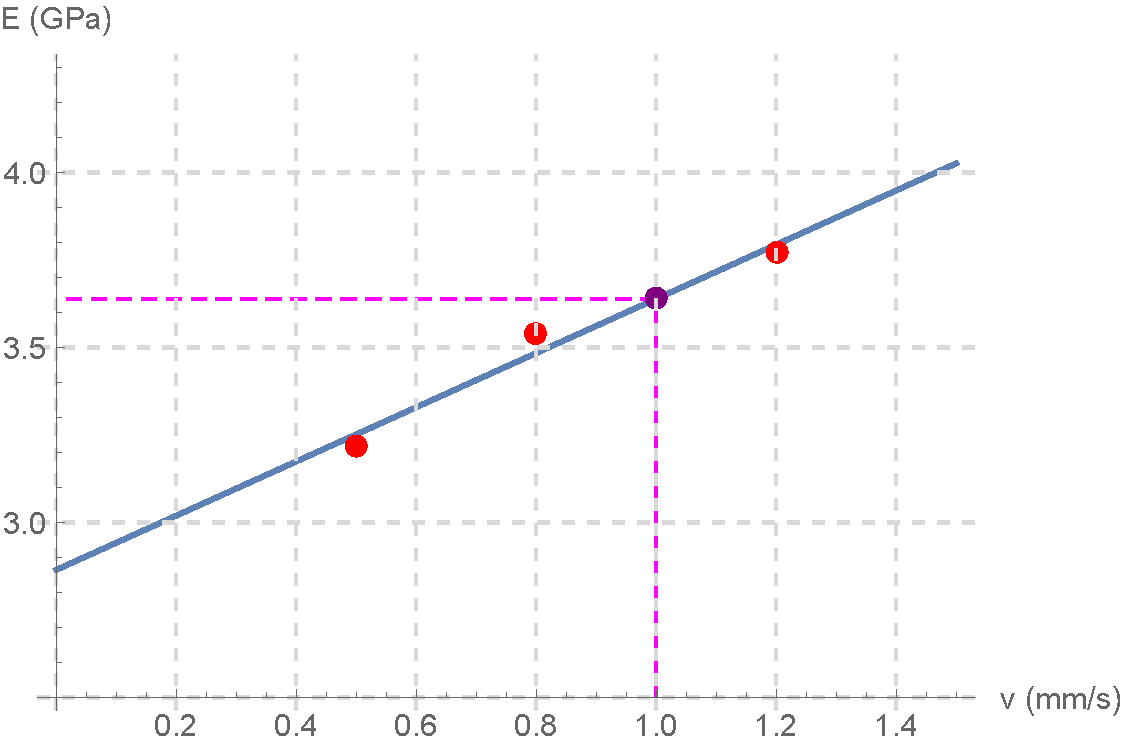
\includegraphics[scale=.6]{images/interpol}
		\caption{Interpolação visando obter o módulo de elasticidade para a velocidade $v=\SI{1}{\milli\meter/\second}$. Nesse caso, a ordenada correspondente é $\textrm{E}=\SI{3.64}{\giga\pascal}$.}
		\label{fig:interpol}
	\end{figure}
	
	\subsection{Equações}
		
	\begin{equation}\label{main_eq}
		\dfrac{\textrm{M}}{\textrm{E}}=\dfrac{1-\nu}{(1+\nu)(1-2\nu)}
	\end{equation}
	
	\begin{equation}\label{strain}
		\nu=-\dfrac{\epsilon_{x}}{\epsilon_{z}}=-\dfrac{\epsilon_{y}}{\epsilon_{z}}
	\end{equation}
	
\end{document}